\FloatBarrier
\Needspace{12\baselineskip}
\section{Пять шагов генерации}

Для диагностики выбраны 256 test-префиксов с пятью последующими
одиночными неорганическими событиями и разрывами до 30 минут.
Все режимы начинают с одной реальной истории и выбирают top-1.
Сравниваются реальный префикс на каждом шаге, добавление каждой
рекомендации, неизменный префикс и эвристика принятия рекомендации

В последнем режиме ID добавляется с вероятностью, равной прогнозу
дослушивания RM. Это допущение о переходе контекста,
которое не проверялось как модель выбора пользователя.
После первого шага NDCG относительно будущего наблюдавшегося объекта
обозначается anchor NDCG. Он показывает отклонение от реальной траектории
и не оценивает контрфактическую релевантность новой политики

\begin{table}[!htbp]
\centering
\small
\setlength{\tabcolsep}{4pt}
\setlength{\reporttablewidth}{\dimexpr\linewidth-32pt\relax}
\begin{tabular}{@{}>{\raggedright\arraybackslash}p{0.34000\reporttablewidth}>{\raggedright\arraybackslash}p{0.18000\reporttablewidth}>{\raggedright\arraybackslash}p{0.16000\reporttablewidth}>{\raggedright\arraybackslash}p{0.16000\reporttablewidth}>{\raggedright\arraybackslash}p{0.16000\reporttablewidth}@{}}
\toprule
Контекст на шаге 5 & Anchor NDCG@10 & Основная RM & Аудитор & KL к реальному \\
\midrule
Реальный префикс & 0.00768 & 0.7710 & 0.7338 & 0.0000 \\
Добавлять каждую рекомендацию & 0.00210 & 0.6916 & 0.7146 & 0.4092 \\
Не менять префикс & 0.00367 & 0.7714 & 0.7358 & 0.2679 \\
Эвристика принятия & 0.00232 & 0.6975 & 0.7176 & 0.3903 \\
\bottomrule
\end{tabular}
\caption{Balanced на срезе непрерывных последовательностей, два столбца RM показывают прогноз дослушивания}
\label{tab:rl-step5}
\end{table}

При добавлении всех рекомендаций anchor NDCG@10 на пятом шаге ниже,
чем с реальным префиксом, распределение выдачи также меняется.
Прогноз дослушивания основной RM падает с 0.7710 до 0.6916.
Накопление искусственного контекста не обеспечивает роста награды
в этом режиме генерации

\begin{figure}[!htbp]
\centering
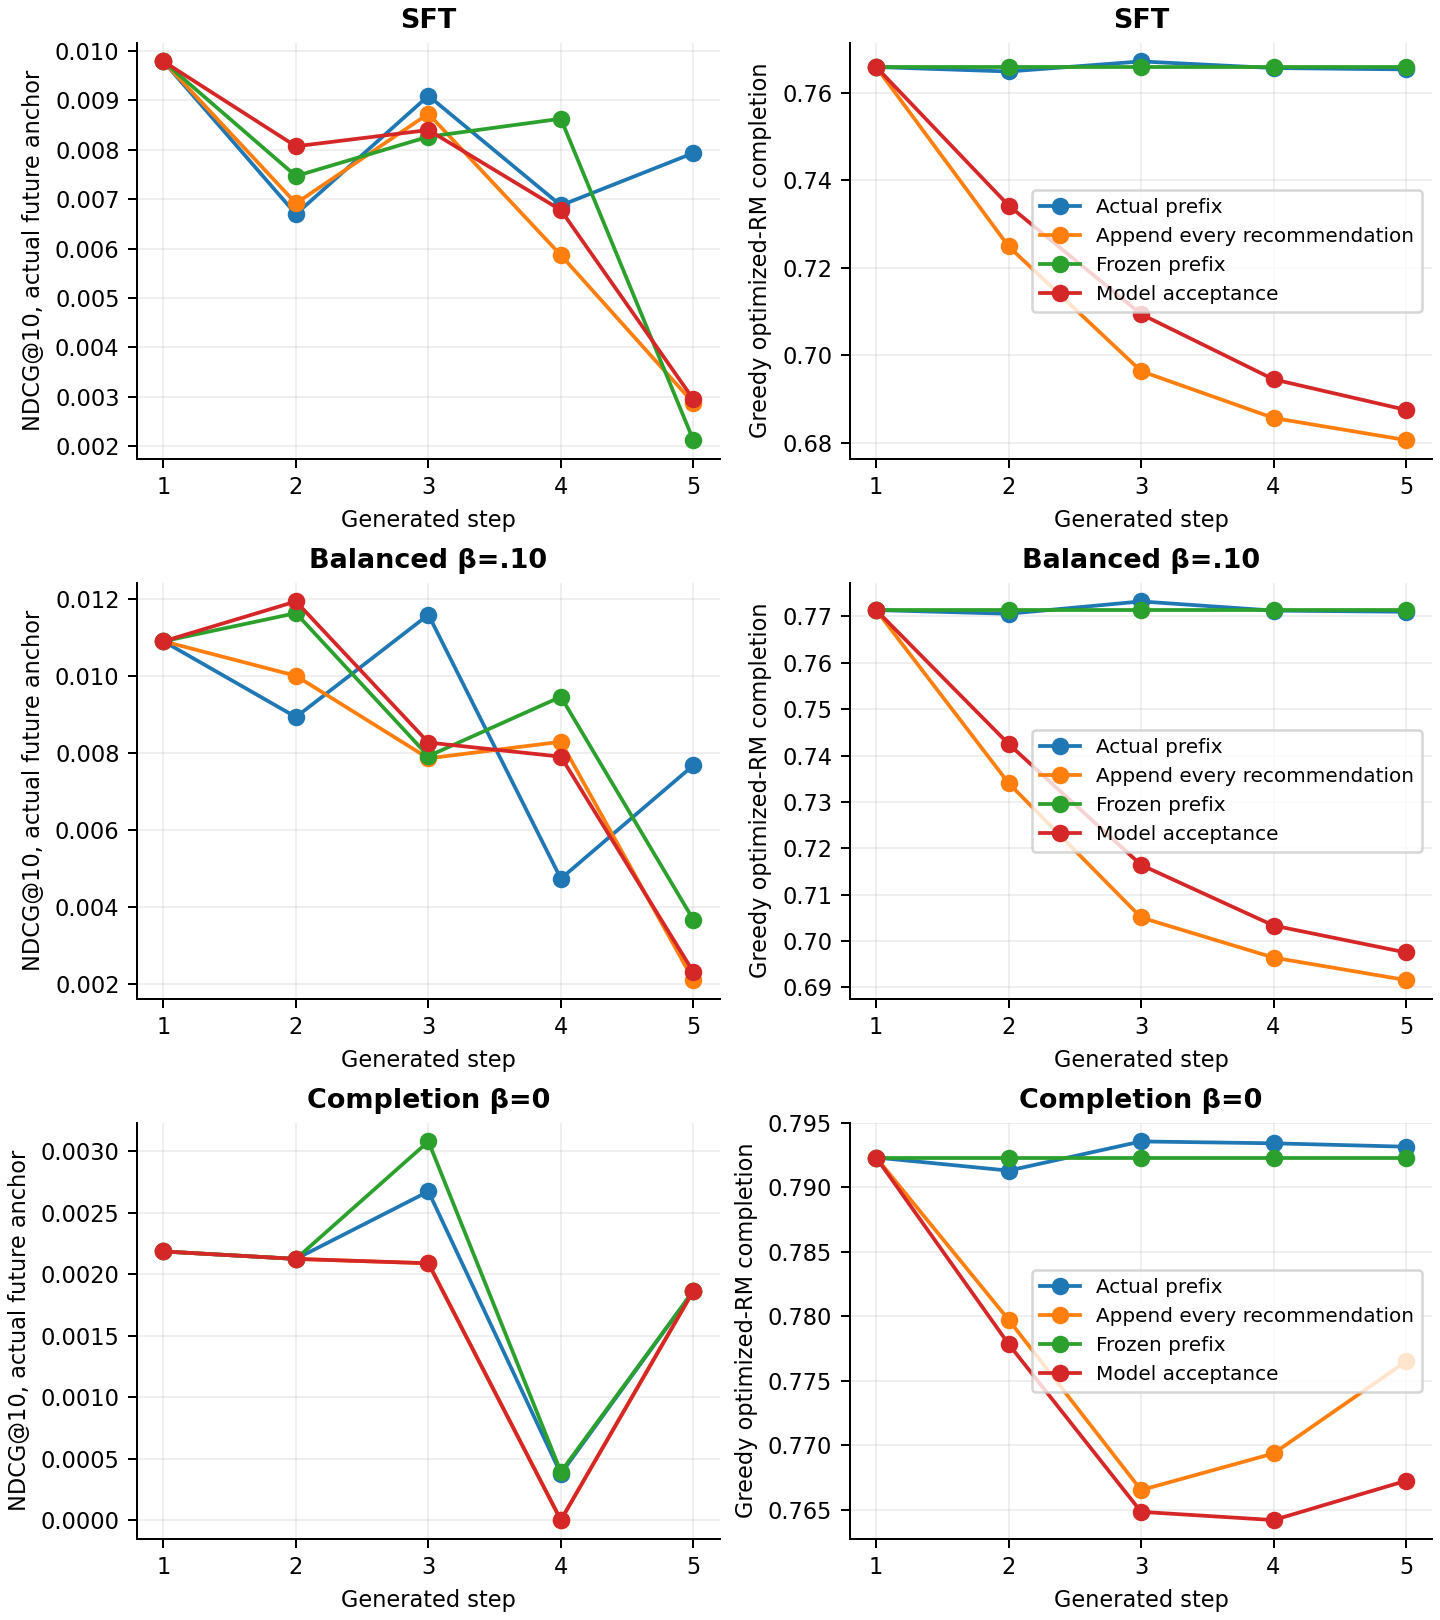
\includegraphics[width=\linewidth,height=.52\textheight,keepaspectratio]{figures/rollouts.png}
\caption{Реальные и искусственные контексты при последовательном выборе top-1}
\label{fig:rl-five-steps}
\end{figure}
